% template-v1.tex: LaTeX2e template for Usenix papers.
% Version: usetex-v1, 31-Oct-2002
% Revision history at end.

\documentclass[finalversion,endnotes]{usetex-v1}
% Choose the appropriate option:
%
% 1. workingdraft:
%
%       For initial submission and shepherding.  Features prominent
%       date, notice of draft status, page numbers, and annotation
%       facilities.  The three supported annotation macros are:
%               \edannote{text}         -- anonymous annotation note
%               \begin{ednote}{who}     -- annotation note attributed
%                 text                          to ``who''
%               \end{ednote}
%               \HERE                   -- a marker that can be left
%                                               in the text and easily
%                                               searched for later
% 2. proof:
%
%         A galley proof identical to the final copy except for page
%         numbering and proof date on the bottom.  Annotations are
%         removed.
%
% 3. webversion:
%
%       A web-publishable version, uses \docstatus{} to indicate
%       publication information (where and when paper was published),
%       and page numbers.
%
% 4. finalversion:
%
%       The final camera-ready-copy (CRC) version of the paper.
%       Published in conference proceedings.  This doesn't include
%       page numbers, annotations, or draft status (Usenix adds
%       headers, footers, and page numbers onto the CRC).
%
% If several are used, the last one in this list wins
%

%
% In addition, the option "endnotes" permits the use of the
% otherwise-disabled, Usenix-deprecated footnote{} command in
% documents.  In this case, be sure to include a
% \makeendnotes command at the end of your document or
% the endnotes will not actually appear.
%

% These packages are optional, but useful
\usepackage{epsfig}     % postscript figures
\usepackage{url}        % \url{} command with good linebreaks

\begin{document}

\title{Experiences with Content Addressable Storage and Virtual Disks}

% document status: submitted to foo, published in bar, etc.
\docstatus{Submitted to Workshop on I/O Virtualization 2008}

% authors.  separate groupings with \and.
\author{
\authname{Anthony Liguori}
\authaddr{IBM Linux Technology Center}
\authurl{\url{aliguori@us.ibm.com}}
\and
\authname{Eric Van Hensbergen}
\authaddr{IBM Research}
\authurl{\url{bergevan@us.ibm.com}}
%
} % end author

\maketitle

\begin{abstract}
Efficiently managing storage is important for virtualized computing 
environments. 
Its importance is magnified by developments such as cloud computing which 
consolidate many thousands of virtual machines (and their associated storage). 
The nature of this storage is such that there is a large amount of 
duplication between otherwise discreet virtual machines. 
Building upon previous work in content addressable storage, we have built a 
prototype for consolidating virtual disk images using a service-oriented file 
system. 
It provides a hierarchical organization, manages historical snapshots of 
drive images, and takes steps to optimize encoding based on partition type and 
file system. 
In this paper we present our experiences with building this prototype and 
using it to store a variety of drive images for QEMU and the Linux
Kernel Virtual Machine (KVM).
\end{abstract}

\section{Motivation}

The installation, organization, and management of disk images is a critical
component of modern virtualization technologies. 
In typical configurations, it is the disk images (and in particular the root
disk image) that defines the identity of a particular virtual machine
instance.
To be effective, a storage virtualization system must be extensible,
able to scale to a large number of virtual machine instances, and support
advanced storage features such as replication, snapshoting, and migration.
It is also highly desirable that such a system be able to rapidly clone
disk images, such that multiple virtual machines may use it as a template
for their own image.

The introduction of cloud computing magnifies the importance
of scalability and efficiency in dealing with storage virtualization.
Instead of dozens of virtual machines, cloud environments are designed
to support thousands (if not hundreds of thousands~\cite{kittyhawk}) of 
virtual machines and so will require many-thousand virtual disk images
in order to function -- as well as sufficient infrastructure to provide
backups and management.

Today's virtualization environments have a variety of mechanisms to 
provide disk images.
Users may use raw hardware partitions physically located on the host's
disks, partitions provided by an Operating System's logical volume 
manager~\cite{lvm}, or partitions accessed via a storage area network.
In addition to these raw partitions, many hypervisors provide copy-on-write
mechanisms which allow base images to be used as read-only templates for 
multiple logical instances which store per-instance modifications.

We have previously experimented with both file and block-based copy-on-write
technologies~\cite{blutopia} for managing the life cycle of servers.
While we found such ``stackable'' technologies to be very effective for
initial installation, the per-instance copy-on-write layers tended to drift.
For example, over the lifetime of the Fedora 7 Linux distribution there 
were over 500MB of software updates to the base installation of 1.8GB.  
While that
represents only about 27\% of changes over a year of deployment -- it becomes
greatly magnified in a large-scale virtualization environment.  

Our assessment at the time was that simple stacking wasn't sufficient,
and that a content addressable storage (CAS) approach to coalescing 
duplicate data between multiple disk images would provide a solution to 
the incremental drift of virtual disks.  
Additionally, the nature of CAS would obviate the
need for end-users to start with a template image as any duplication would
be identified and addressed by the CAS back end.
Furthermore, CAS solutions lend themselves to rapid cloning, snapshoting,
and can be configured to implicitly provide temporal-based backups of images.

Others have looked at using CAS solutions for archival of virtual machine
images~\cite{foundation} and managing disk images~\cite{mirage}.  
Nath, et.al. evaluate the use and design tradeoffs of CAS
in managing a large set of VM-based systems in an enterprise 
environment~\cite{nath}.
In all of these cases, the authors used content addressable storage as a 
sort of library from which disk images could be ``checked-out''.  
We were more interested in looking at a \emph{live} solution where the 
disk image was always directly backed by content addressable storage such 
that no check-in or check-out transactions are necessary. 

The rest of this paper is organized as follows: section 2 provides the results
of our preliminary analysis comparing the amount of duplication present in
several loosely related disk images.
Section 3 describes our prototype implementation of a content addressable
image management system for virtual machines.
Section 4 gives our preliminary performance analysis of the prototype,
and section 5 describes our status and future work.

\section{Image Analysis}

In order to assess the potential for coalescing duplicated data between
virtual disk images we compared a cross-section of images from various 
versions of various Linux distributions as well images resulting from
separate installs of Windows XP.
We establish overlap candidates by crawling the file systems, producing a SHA-1
cryptographic hash for each file and associating it with the size of the 
file and the number of hard-links to the file in a manner similar to
Mirage's manifests~\cite{mirage}.
The Linux file systems in question are Ext2 formatted root volumes
(without /boot which contains the kernels and ram disks) present after the 
default installation of the various distributions.

We then determine the amount of self-similarity within a file system by looking
for duplicate hashes and discounting hard linked copies as false duplicates.
Our analysis showed that typical root disk images have around 5\% 
duplicate file data within a single image after initial installation, 
and that the amount of duplicate file data seems to be increasing 
(Fedora 7 had 4.1\% or 70MB, Fedora 9 has 5.3\% or 116MB).
We then concatenate file lists from two different images and look for
duplicate file hashes to establish the amount of data duplicated between
the two images.  The total size of the duplicate files is compared to the
total size of all files from the two images to calculate the \% of duplicates.

\begin{figure}[htbp]
\begin{centering}
\begin{tabular}{|l|r|r|r|r|}	\hline 
\emph{Image}	& Base	& Office	& SDK	& Web \\ \hline
Base	& 96\%	& 88\%	& 85\%	& 95\% \\
Office	& 	& 96\%	& 79\%	& 87\% \\
SDK	& 	& 	& 96\%	& 85\% \\
Web	& 	& 	& 	& 96\% \\	\hline
\end{tabular}
\small\itshape
\caption{\small\itshape Different Fedora 9 Flavors}
\label{fig:flavors}
\end{centering}
\end{figure}

Figure~\ref{fig:flavors} shows the amount of similarity between
separate installs of several different configurations of the Fedora 9
x86--64 distribution.  The image personality is determined by options
selected during the installation process.
The \emph{Base} configuration is the 
standard installation, with no personality configuration selected.
The \emph{Office} configuration contains productivity applications such
as OpenOffice, the \emph{SDK} configuration contains development tools
and resources, and the \emph{Web} configuration contains the necessary
applications for web serving.
Separate installations of the same configuration had 96\% similarity 
according to our methodology.  The differences are likely log files and
other metadata which would be particular to a specific system instance.
Not surprisingly, the similarity amongst the different configurations is 
relatively high due to the common base installation which accounts for 
around 80\% or more of the data.

\begin{figure}[htbp]
\begin{centering}
\resizebox{\columnwidth}{!}
{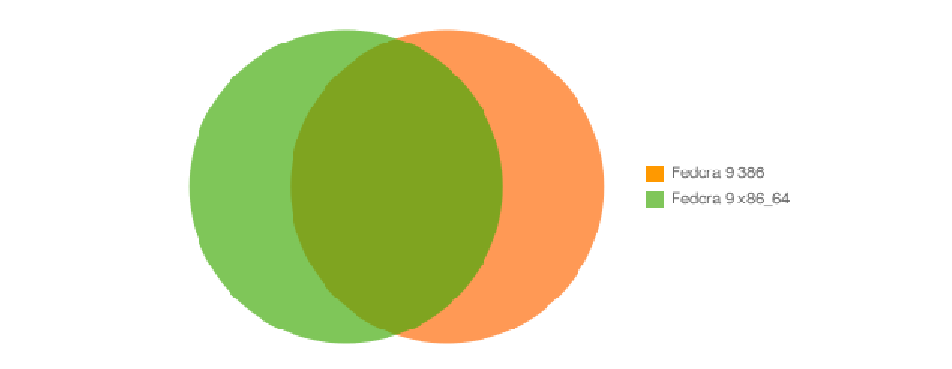
\includegraphics{fedorax86}}
\small\itshape
\caption{\small\itshape Different Architectures}
\label{fig:arch}
\end{centering}
\end{figure}

We then compared slightly less similar images by
comparing the installation of a 32-bit Fedora 9 system with
a 64-bit Fedora 9 system.  As can be seen in Figure~\ref{fig:arch}
we observed roughly 60\% overlap between the two images consisting 
primarily of the non-binary portions of the installation (configuration
files, fonts, icons, documentation, etc.).

\begin{figure}[htbp]
\begin{centering}
\begin{tabular}{|l|r|r|r|r|r|}	\hline 
\emph{Image}	& Fed 8	& Fed 9	& Ubuntu	& OpenSuSe-11	\\ \hline
Fedora 7 	& 34\%	& 22\%	&  8\%	& 15\% \\
Fedora 8 	& 	& 31\%	& 10\%	& 16\% \\
Fedora 9	& 	& 	& 11\%	& 21\% \\
Ubuntu 8.04	& 	& 	& 	& 8\% \\	\hline
\end{tabular}
\small\itshape
\caption{\small\itshape Different Distributions}
\label{fig:distro}
\end{centering}
\end{figure}

Next, we compared several different distributions, looking at the overlap
between different versions of Fedora as well as 32-bit versions of
Ubuntu and OpenSuSe 11.
The resulting overlap can be seen in Figure~\ref{fig:distro}. 
As one might expect, adjacent versions of the distribution had relatively
high degrees of overlap ranging from 22\% to 34\% despite about a year of
time between their respective releases.
It should be pointed out that the effect is cumulative, if looking across 
all three distributions which total about 6 GB of root file system data, 
2GB of that data is overlapped data resulting in approximately 1.2GB of
wasted space.
The overlap between the Fedora installations and the other distribution
vendors is less striking.  There was a high degree of overlap between 
Fedora and OpenSuSe but a much lower degree of overlap with Ubuntu.
The results are a little offset because the Ubuntu image is almost an
order of magnitude smaller than the Fedora and SuSe base installations.

\begin{figure}[htbp]
\begin{centering}
\resizebox{\columnwidth}{!}
{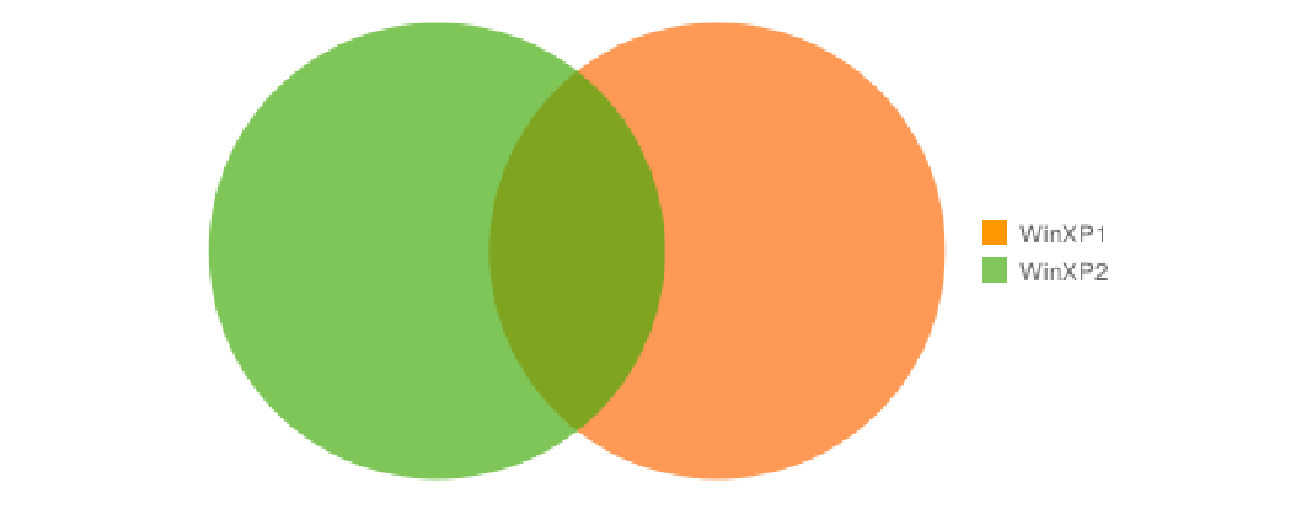
\includegraphics{winxp}}
\small\itshape
\caption{\small\itshape Individual WindowsXP Installs}
\label{fig:windows}
\end{centering}
\end{figure}

Switching from Linux to Windows, we compared two separate installations
of WindowsXP on a FAT32 file system. 
We selected a FAT32 installation over NTFS to reduce the complexity of
analyzing block-based results.
We were somewhat dismayed to discover only a 27\% overlap as can be seen
in Figure~\ref{fig:windows}.
A closer look reveals that the two largest files in the instance file systems
are the hibernation file (\emph{hiberfil.sys}) clocking in at just under
a gigabyte in size and the swap file (\emph{pagefile.sys}) hovering around
1.5 gigabytes in size.  This 2.5 gigabytes actually comprises more then 60\%
of the overall size of the file system.  Discounting these two files we find
roughly 90\% overlap between the two distributions.

\begin{figure}[htbp]
\begin{centering}
\resizebox{\columnwidth}{!}
{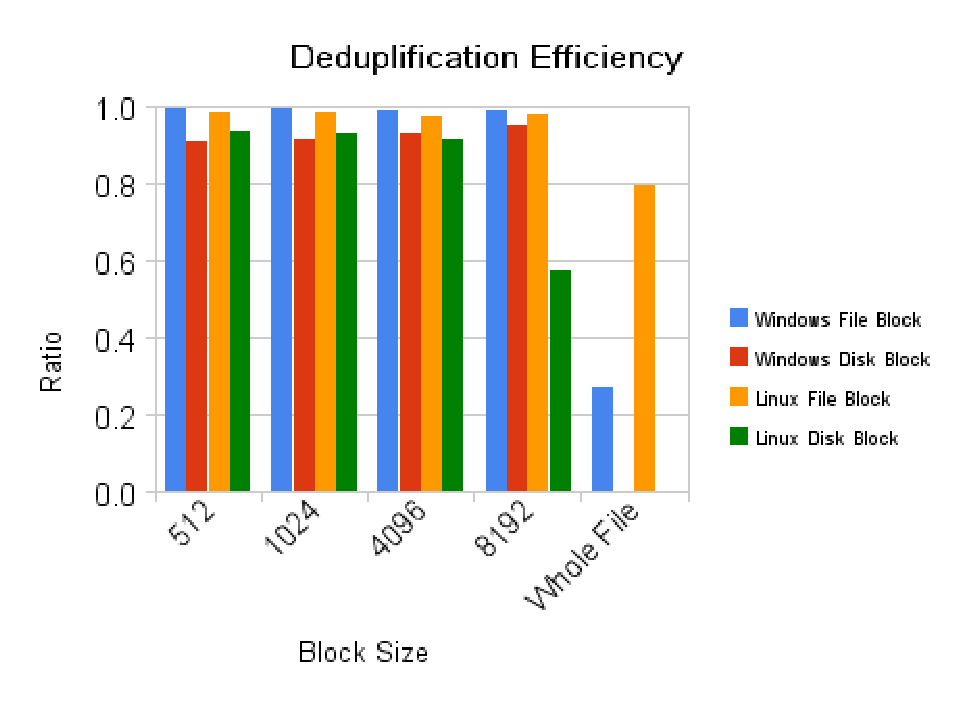
\includegraphics{deduplification_efficiency}}
\small\itshape
\caption{\small\itshape Effect of Block Size on Efficiency}
\label{fig:block}
\end{centering}
\end{figure}

Digging deeper, we observed that both of these files were primarily 
zero--filled.
We reworked our analysis tools to perform block-level hashing of files
within the file system at 512-byte, 1k, 4k, and 8k granularities.
By comparing file content hashes at this level of granularity we were
able to more effectively detect duplication within files as well as 
handle sparse files more efficiently.  As can be seen in the 
\emph{Windows File Block} results in Figure~\ref{fig:block} we achieved near
perfect (99\%) de-duplification of the two Windows install images using
any of the block size options.  Results were fractional better with 512
byte blocks, but the overhead associated with tracking such small blocks
in a CAS would far outweigh the benefits.

We also used the same tool to scan the raw disk image at the
various block granularities.  Its effectiveness at de-duplicating blocks
are shown in the \emph{Windows Disk Block} result in Figure~\ref{fig:block}.
The results show a slightly higher efficiency for 8k blocks, but this is
primarily due to error associated with partial blocks and our discounting
zero-filled-blocks.  The disk based scan was able to identify approximately
93\% of the duplicate data.

We then applied these same two techniques to analyzing two different
installations of the same Linux distribution as can be seen in the
\emph{Linux File Block} and \emph{Linux Disk Block} results.  We found
similar results to the Windows analysis with the exception that 8k
block granularity did very poorly with Linux most likely due to differences
between Ext2 and FAT32 layout schemes since both file systems reported using
4k block sizes.


\section{Implementation}

In order to get a better idea of the performance and efficiency implications 
of using a CAS based image management system, we constructed a prototype by
combining the Venti~\cite{venti} CAS back end with a service-oriented file 
system to provide an organizational infrastructure and tested it with 
guest logical partitions running under QEMU~\cite{qemu} which provides the
Virtual I/O infrastructure for KVM~\cite{kvm}. 

Venti provides virtualized storage which is addressed via SHA-1 hashes.
It accepts blocks from 512 bytes to 56kb, using hash trees of blocks to
represent larger entries (VtEntry), and optionally organizing these entries in 
hash trees of hierarchical directories (VtDir), which are collected into
snapshots represented by a VtRoot structure.
Each block, VtEntry, VtDir, and VtRoot has an associated hash value, which 
is also referred to as a score.  
Venti maintains an index which maps these scores to physical disk blocks
which typically contain compressed versions of the data they represent.
Since the SHA-1 hash function effectively summarizes the contents of the
block, duplicate blocks will resolve to the same hash index -- allowing 
Venti to coalesce duplicate data to the same blocks on physical storage.

Using Venti to store partition images is as simple as treating the partition
as a large VtEntry.
Slightly more intelligent storage of file system data (to match native block
sizes and avoid scanning empty blocks) can be done with only rudimentary 
knowledge of the underlying file system.
If the file system isn't recognized, the system can fall-back to a default
block size of 4k.
This approach is used by the vbackup utility in 
Plan 9 from User Space~\cite{plan9ports} which can be used to provide 
temporal snapshots of 
typical UNIX file systems, and is also used by Foundation~\cite{foundation}
which provides archival snapshots of VMware disk images.
Multi-partition disks can be represented as a simple one level directory 
with a single VtEntry per partition.  

Venti only presents an interface to retrieving data by scores and doesn't
provide any other visible organizational structure.  
To address this, we built vdiskfs, a stackable synthetic file server which 
provides support for storing and retrieving disk images in Venti.
Currently, it is a simple pass-through file server that recognizes special
files ending in a ``.vdisk'' extension. 
In the underlying file system a ``.vdisk'' file contains the SHA-1 hash that 
represents a Venti disk image snapshot.  
When accessed via vdiskfs, reads of the file will expose a virtual raw image
file.
vdiskfs is built as a user-space file system using the 9P protocol which can
be mounted by the Linux v9fs~\cite{graverobber} kernel module or accessed 
directly by applications.

QEMU internally implements an abstraction for block device level I/O through 
the BlockDriverState API.  
We implemented a new block device that connects directly to a 9P file server.  
The user simply provides the host information of the 9P
file server along with a path within the server and QEMU will connect to 
the server, obtain the size of the specified file, and direct all read/write 
requests to the file server.

In communicating directly to the 9P file server, QEMU can avoid extraneous data
copying that would occur by first mounting the file system in the host with a
synthetic file system.  It also avoids double-caching the data in the host's
page cache.  Consider a scenario where there were two guests both sharing the
same underlying data block.  This block will already exist once in the host's
page cache when Venti reads it for the first time.  If a v9fs mount was created
that exposed multiple images that contained this block, whenever a user space
process (like QEMU) read these images, a new page cache entry would be added for
each image.

While QEMU can interact directly with the 9P file server, there is a great 
deal of utility in having a user-level file system mount of the synthetic 
file system.  
Virtualization software that is not aware of 9P can open these images directly 
paying an additional memory/performance cost.  
A user can potentially import and export images easily using traditional 
file system management utilities (like cp).  

We used QEMU/KVM as the virtual machine monitor in our implementation.  
QEMU is a system emulator that can take advantage of the Linux Kernel Virtual 
Machine (KVM) interface to achieve near-native performance.  
All I/O in QEMU is implemented in user space which makes it particularly well 
suited for investigating I/O performance.

QEMU/KVM supports paravirtual I/O with the VirtIO~\cite{virtio} framework.  
VirtIO is a simple ring-queue based abstraction that minimizes the number of 
transitions between the host and guest kernel.  
For the purposes of this paper, we limited our analysis to the emulated 
IDE adapter within QEMU/KVM.  
VirtIO currently only achieves better performance for block I/O in 
circumstances where it can issue many outstanding requests at a time.  
The current vdiskfs prototype can only process a single request at a time.  
Moreover, QEMU is also limited in its implementation to only support a 
single outstanding request at a time.

\section{Performance}

Our performance tests were done using QEMU/KVM on a 
2-way AMD Quad-core Barcelona system with 8GB of
RAM and a 13 disk fibre channel storage array. Venti
was configured with a 10GB arena and a 512MB isect
and bloom filter. Venti was configured with 32MB of
memory cache, a 32MB bloom cache, and a 64MB isect cache.

For each of our benchmarks, we compared an image
in an Ext3 file system using the QEMU raw block driver
back end, an image exposed through ufs, a user space 9P
file server, using the QEMU block-9P block driver back
end, and then an image stored in Venti exposed through
vdiskfs using the QEMU block-9P block driver back end.

Each benchmark used a fresh Fedora 9 install for
x86\_64. For all benchmarks, we backed the block driver
we were testing with a temporary QCOW2 image. The 
effect of this is that all writes were thrown away. This was
necessary since vdiskfs does not currently support write
operations.

Our first benchmark was a simple operating system
boot measured against wall clock time. The purposes of
this benchmark was to determine if a casual user would
be impacted by the use of a content addressable storage
backed root disk.
Our measurements showed that the when using the QEMU
block-9P driver against a simple 9P block server, there
was no statistically significant difference in boot time
or CPU consumption compared to the QEMU raw block driver.
When using the QEMU block-9P driver against vdiskfs,
we observed a 25% slowdown in boot time along with a 20%
reduction in CPU consumption due to increased latency for
I/O operations.

\begin{figure}[htbp]
\begin{centering}
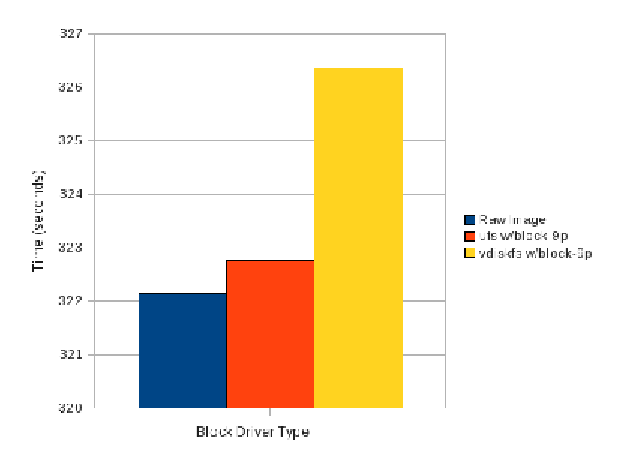
\epsfig{file=bootup.eps, width=2.50in}
\small\itshape
\caption{\small\itshape Boot Time of CAS Storage}
\label{fig:bootup}
\end{centering}
\end{figure}

The second benchmark was a timed \emph{dd} operation.
The transfer size was 1MB and within the guest, direct
I/O was used to eliminate any effects of the guest page
cache. It demonstrates the performance of streaming
read. All benchmarks were done with a warm cache so the
data is being retrieved from the host page cache.

The ufs back end is able to obtain about 111MB/sec using
block-9P.  Since all accesses are being satisfied by the
host page cache, the only limiting factor are additional
copies within ufs and within the socket buffers.

The QEMU raw block driver is able to achieve over
650MB/sec when data is accessed through the host page cache.
We believe it is possible to achieve performance similar to
the QEMU raw block driver through ufs by utilizing splice
in Linux.

\begin{figure}[htbp]
\begin{centering}
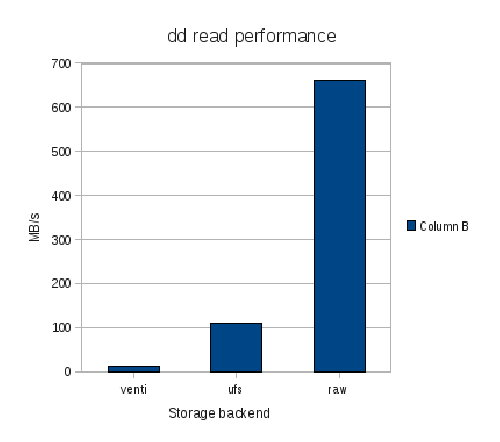
\epsfig{file=dd.eps, width=2.50in}
\small\itshape
\caption{\small\itshape Streaming Read Performance}
\label{fig:streamingread}
\end{centering}
\end{figure}

vdiskfs is only able to obtain about 12MB/sec using
block-9P. 
While this performance may seem disappointing, it
is all we expected from the existing implementation
of Venti and we talk about some approaches to improving
it in Section 5.

\begin{figure}[htbp]
\begin{centering}
\resizebox{\columnwidth}{!}
{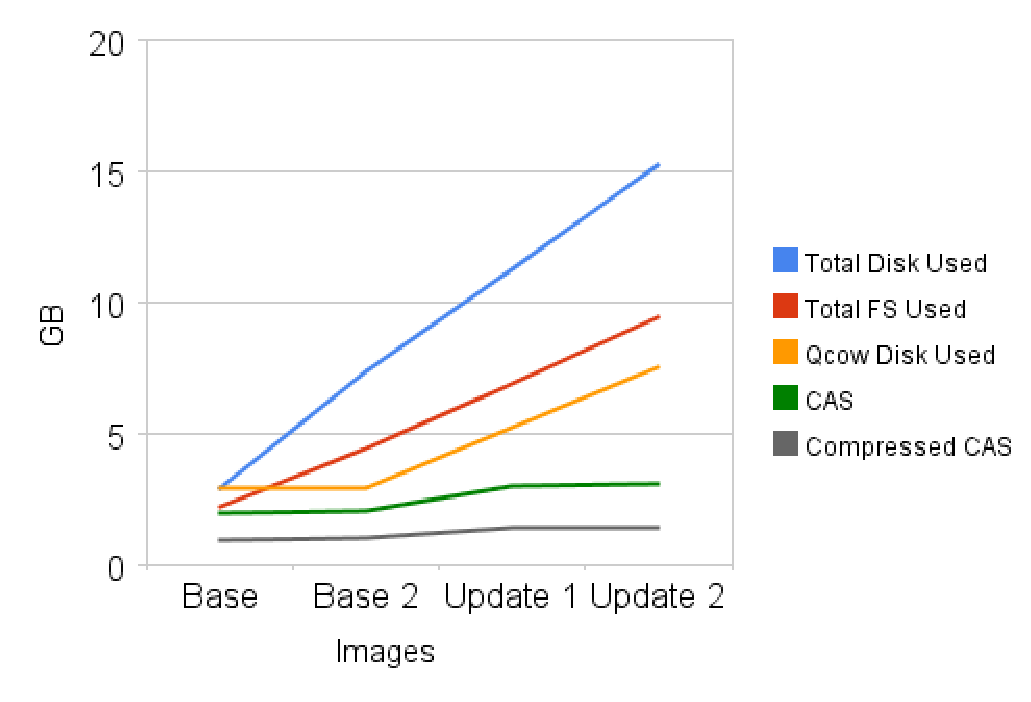
\includegraphics{venti_analysis}}
\small\itshape
\caption{\small\itshape Efficiency of Underlying Storage Technique}
\label{fig:venti}
\end{centering}
\end{figure}

Finally, to validate whether or not content addressable storage schemes
would improve storage efficiency in the face of software-updates we compared
the disk overhead of two instances of a Linux installation before and after
a software update.  We compared raw disk utilization, file system reported
space used, copy-on-write image disk utilization, content addressable storage,
and compressed content addressable storage.
To construct the copy-on-write images, we used the QEMU QCOW2 format and
used the same base image for both \emph{Base} and \emph{Base2}.
To evaluate the content addressable storage efficiency we used Venti to
snapshot the raw disk images after installation and again after a manual
software update was run.  We used Venti's web interface to collect data about
its storage utilization for compressed data as well as its projections for
uncompressed data.

As can be seen in Figure~\ref{fig:venti} the various solutions all take
approximately the same amount of storage for a single image.  When adding
a second instance of the same image, the raw storage use doubles while both
the copy-on-write storage and content-addressable-storage essentially remain
the same.
The software update process on each image downloaded approximately 500MB of 
data.  As the update applied, each QCOW2 image (as well as the raw disk
images) increased in size proportionally.

We were surprised to find both the raw disk and copy-on-write overhead for the
software update was over double what we expected.  
We surmise this is due to temporary files and other transient data written
to the disk and therefore the copy-on-write layer.
This same dirty-but-unused block data is also responsible for the 
divergence between the \emph{Total FS Used} and the \emph{Total Disk Used} 
lines in the reported storage utilization.
This behavior paints a very bad efficiency picture for copy-on-write 
solutions in the long term.
While copy-on-write provides some initial benefits, their storage utilization
will steadily increase and start to converge with the amount of
storage used by a raw-disk installation.

Utilizing the disk block scanning techniques we applied in Section 2, we
found we could detect and de-duplicated these transient dirty blocks.
Such an approach may work to improve overall performance once we work out
the scalability and performance issues of the underlying CAS mechanism.
Because Venti is partially aware of the underlying structure of the Ext2
file system it only snapshots active file blocks.  
As a result, its storage utilization grows slightly for the
first software update, but the overhead of the second software update is
completely eliminated. 


\section{Future Work}

While we have shown promising efficiency improvements, it is clear that the
current Venti performance in this environment is far below what would be
desirable.
Venti was primarily developed as a backup archive server, and as such its
implementation is single threaded and not constructed to scale under
heavy load.
Additionally, its performance is primarily bottlenecked by the requirement
of indirecting block requests via the index which results in random access
by the nature of the hash algorithm~\cite{memventi}.
In our future work we plan to address these issues by reworking the Venti
implementation to support multi-threading, more aggressive caching, and
zero-copy of block data.
The use of flash storage for the index may further diminish the additional
latency inherent in the random-access seek behavior of the hash lookup.

Our target environment will consist of a cluster of collaborating 
Venti servers which provide the backing store for a 
larger cluster of servers acting as hosts for virtual machines.  
In addition to our core Venti server optimizations, we wish to employ
copy-on-read local disk caches on the virtual machine hosts to hide 
remaining latency from the guests.
We also plan on investigating the use of collaborative caching environments
which will allow these hosts and perhaps even the guests to share each other's 
cache resources.

Another pressing area of future work is to add write support to vdiskfs to
allow end-users to interact with it in a much more natural manner.
We plan on employing a transient copy-on-write layer which will buffer
writes to the underlying disk.  
This write buffer will routinely be flushed to Venti and the vdisk score
updated.
Venti already maintains a history of snapshot scores through links in the 
VtRoot structure, so historical versions of the image can be accessed at later
times.
We would also like to provide a synthetic file hierarchy to access snapshots
in much the same way as implemented by Plan 9's yesterday command.

Linux recently added a series of system calls to allow user space applications 
to directly manipulate kernel buffers known as splice.  
The splice system call could be used by a 9P file server to move data 
directly from the host page cache, into a kernel buffer, and then allow 
the actual client application (such as QEMU's block-9P back end) to copy the 
data directly from the kernel buffer into its memory.  
In this way, we can avoid the additional copy to and from the TCP socket buffer.

Another area to explore is to look at integrating the content addressable
storage system with an underlying file system to see if we can obtain 
efficiency closer to that of what we measured using our file-system crawling
mechanism.
We could use our paravirtualized 9P implementation to allow direct access
to the file system from the guests instead of using virtual block devices.
This would eliminate some of the extra overhead, and may provide a better
basis for cooperative page caches between virtual machines.
It also provides a more meaningful way for a user to interact with the 
guest's file system contents than virtual images provide.

While the large performance gap represents a particularly difficult challenge, 
we believe that the efficiency promise of content addressable storage for 
large scale virtual machine environments more than adequately justifies 
additional investment and investigation in this area.


\bibliographystyle{plain}
\bibliography{references}

\end{document}

% Revision History:
% designed specifically to meet requirements of
%  TCL97 committee.
% originally a template for producing IEEE-format articles using LaTeX.
%   written by Matthew Ward, CS Department, Worcester Polytechnic Institute.
% adapted by David Beazley for his excellent SWIG paper in Proceedings,
%   Tcl 96
% turned into a smartass generic template by De Clarke, with thanks to
%   both the above pioneers
% use at your own risk.  Complaints to /dev/null.
% make it two column with no page numbering, default is 10 point

% Munged by Fred Douglis <douglis@research.att.com> 10/97 to separate
% the .sty file from the LaTeX source template, so that people can
% more easily include the .sty file into an existing document.  Also
% changed to more closely follow the style guidelines as represented
% by the Word sample file.
% This version uses the latex2e styles, not the very ancient 2.09 stuff.
%

% Revised July--October 2002 by Bart Massey, Chuck Cranor, Erez
% Zadok and the FREENIX Track folks to ``be easier to use and work
% better''. Hah.  Major changes include transformation into a
% latex2e class file, better support for drafts, and some
% layout improvements.
%%%%%%%%%%%%%%%%%%%%%%%%%%%%%%%%%%%%%%%%%%%%%%%%%%%%%%%%%%%%%%%%%%%%%%%%%%%%%%
% for Ispell:
% LocalWords:  workingdraft BCM ednote SubSections xfig SubSection joe
